 %%%%%%%%%%%%%%%%%%%%%%%%%%%%%%%%%%%%%%%%%%%%%%%%%%%%%%%%%%%%%%%%%%%%%%%%%%%%%%%%
%2345678901234567890123456789012345678901234567890123456789012345678901234567890
%        1         2         3         4         5         6         7         8

\documentclass[letterpaper, 10 pt, conference]{ieeeconf}  % Comment this line out if you need a4paper

%\documentclass[a4paper, 10pt, conference]{ieeeconf}      % Use this line for a4 paper

\IEEEoverridecommandlockouts                              % This command is only needed if 
                                                          % you want to use the \thanks command

\overrideIEEEmargins                                      % Needed to meet printer requirements.

%In case you encounter the following error:
%Error 1010 The PDF file may be corrupt (unable to open PDF file) OR
%Error 1000 An error occurred while parsing a contents stream. Unable to analyze the PDF file.
%This is a known problem with pdfLaTeX conversion filter. The file cannot be opened with acrobat reader
%Please use one of the alternatives below to circumvent this error by uncommenting one or the other
%\pdfobjcompresslevel=0
%\pdfminorversion=4

% See the \addtolength command later in the file to balance the column lengths
% on the last page of the document

% The following packages can be found on http:\\www.ctan.org
\usepackage{graphicx} % for pdf, bitmapped graphics files
%\usepackage{epsfig} % for postscript graphics files
%\usepackage{mathptmx} % assumes new font selection scheme installed
%\usepackage{times} % assumes new font selection scheme installed
\usepackage{amsmath} % assumes amsmath package installed
%\usepackage{amssymb}  % assumes amsmath package installed
\usepackage{url}
\usepackage{gensymb}

\title{\LARGE \bf
COMP 551 Kaggle Competition: Classification of Modified MNIST*
}


\author{Yingnan Zhao$^{1}$, Vincent d'Orsonnens$^{2}$ and Hamed Layeghi$^{3}$% <-this % stops a space
\thanks{*Kaggle Team name: BetaGo, Best Score: 0.95899}% <-this % stops a space
\thanks{$^{1}$Yingnan Zhao, Student ID: 260563769, Electrical Engineering, 
        McGill University,
        {\tt\small nan.zhao2@mail.mcgill.CA}}%
\thanks{$^{2}$Vincent d'Orsonnens, Student ID: 260746099, Software Engineering, McGill University, 
        {\tt\small vincent.dorsonnens@mail.mcgill.ca}}%
\thanks{$^{3}$Hamed Layeghi, Student ID: 260524499, Electrical Engineering, McGill University, 
	{\tt\small hamed.layeghi@mail.mcgill.ca}}%
}

\begin{document}



\maketitle
\thispagestyle{empty}
\pagestyle{empty}


%%%%%%%%%%%%%%%%%%%%%%%%%%%%%%%%%%%%%%%%%%%%%%%%%%%%%%%%%%%%%%%%%%%%%%%%%%%%%%%%
\begin{abstract}
This paper provides the report for the Kaggle Competition (assignment 4) of COMP 551 using the provided Modified MNIST dataset. The dataset includes a set of 8-bit grayscale images that include 2 or 3 digits of different sizes that are rotated and scaled from the classic MNIST dataset. The goal is to design Machine Learning algorithms that identify the biggest digit in each image. Several algorithms have been used in the report. First, a linear SVM is used which lead to relatively low accuracy. Second, a fully connected neural network completely developed by the team was implemented. Finally, a convoluted neural network was trained and tested on the preprocessed dataset which showed the best performance.  
\end{abstract}


%%%%%%%%%%%%%%%%%%%%%%%%%%%%%%%%%%%%%%%%%%%%%%%%%%%%%%%%%%%%%%%%%%%%%%%%%%%%%%%%
\section{INTRODUCTION}

The MNIST database \cite{MNISTcreators} is a set of handwritten images that is popular for training and testing of Machine Learning algorithms \cite{wiki:MNIST}.

\section{PREPROCESSING}
The provided images in the Modified MNIST include 3 numbers that are rotated and scaled from the MNIST dataset and are written on random backgrounds.
Some samples of the train dataset with their associated outputs are shown in Figure \ref{fig:original}.
\begin{figure}[h]
	\begin{center}
		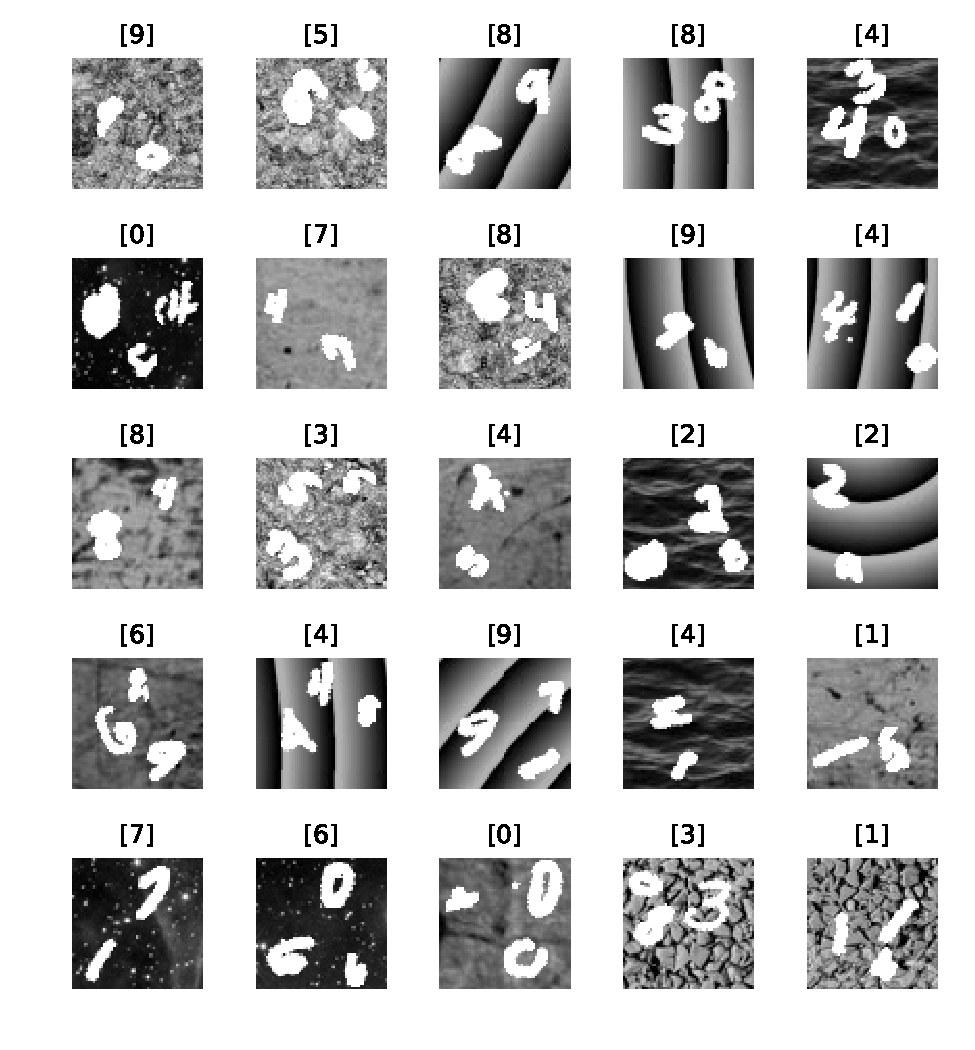
\includegraphics[width=0.5\textwidth]{figures/originalDataset.pdf}  % The printed column width is 8.4 cm.
		\caption{25 Random Samples of the original train dataset}
		\label{fig:original}
	\end{center}
\end{figure}

 The format for the images is 8-bit grayscale image, thus each pixel has 256 shades of gray represented by numbers 0 (black) to 255 (white) as shown in Figure \ref{fig:maxeig2}.

	
\begin{figure}[h]
	\begin{center}
			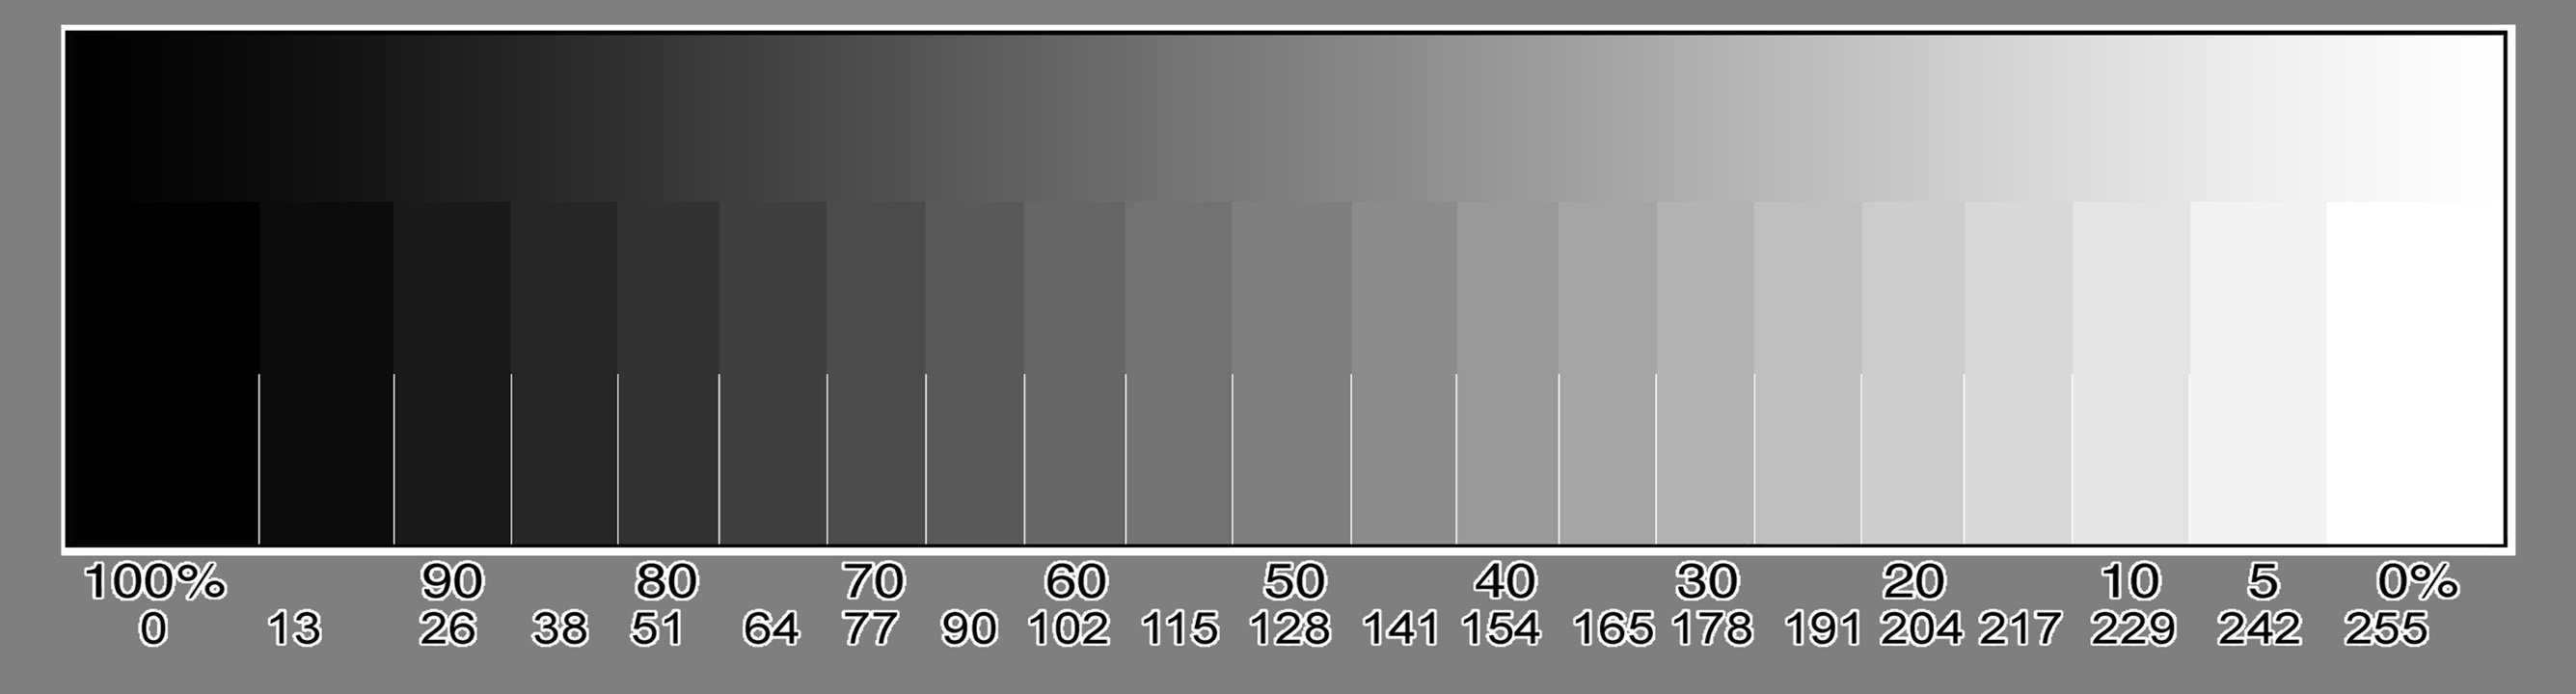
\includegraphics[width=0.5\textwidth]{figures/21stepwide8bit.jpg}  % The printed column width is 8.4 cm.
		\caption{8-bit Grayscale Shades of Gray}
		\label{fig:maxeig2}
	\end{center}
\end{figure}

Before, the data are used for training, the following preprocessing steps are used.

\subsection{Thresholding} 
Since the numbers in the dataset match the 255 shade, a simple idea for preprocessing is to use \textit{image thresholding}. 
The idea of thresholding is to compare the pixel values of the input image $f$ with some threshold $T$ and make a binary decision for the output binary image $g$ as below
\begin{align}
g(i,j) = \begin{cases}
1 & f(i,j)\ge T\\
0 & f(i,j)\le T
\end{cases}
\end{align}
for all $i, j$ where $i, j$ represent the coordinates of the $ij$\textsuperscript{th} pixel \cite{bovik2009essential}.

The output of this filter is shown in Figure \ref{fig:thresholded}

\begin{figure}[h]
	\begin{center}
		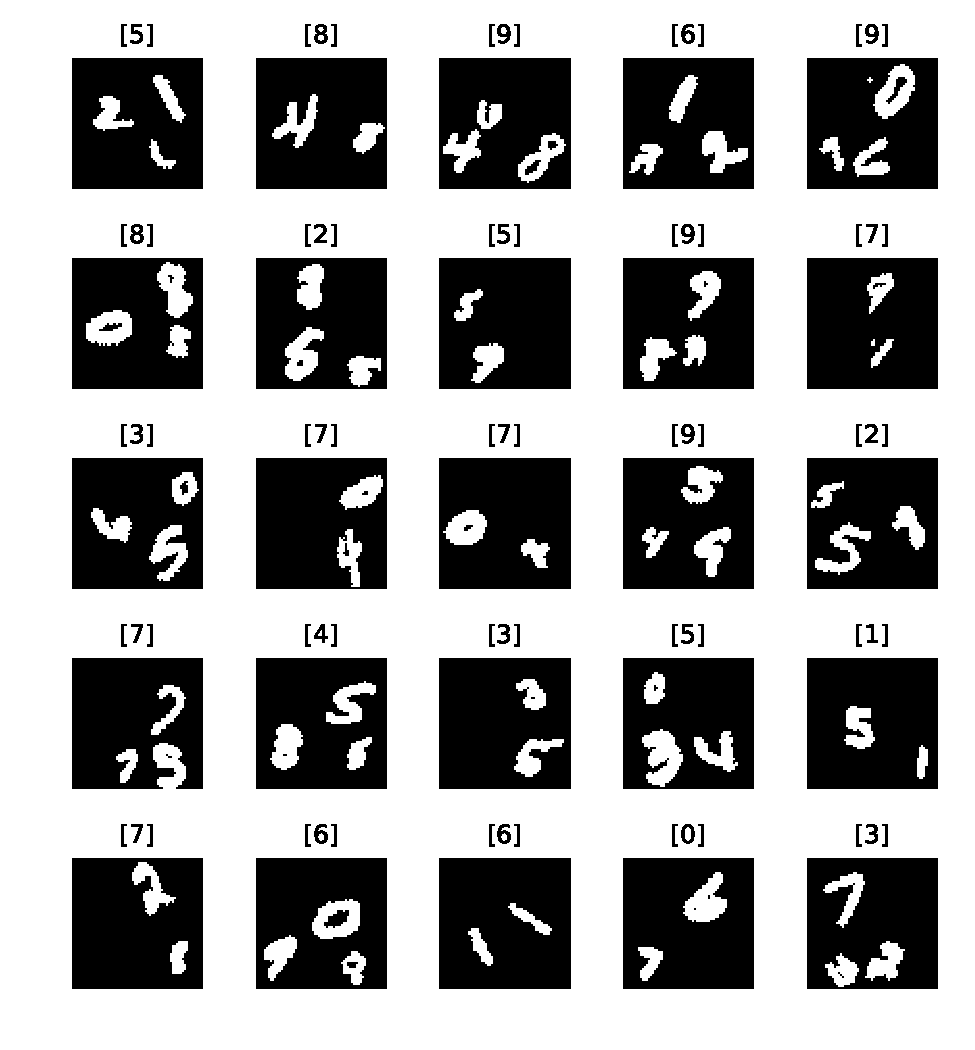
\includegraphics[width=0.5\textwidth]{figures/thresholdDataset.pdf}  % The printed column width is 8.4 cm.
		\caption{Output of thresholding on images from Figure \ref{fig:original}}
		\label{fig:thresholded}
	\end{center}
\end{figure}

\subsection{Median Filter}
As can be seen in Figure \ref{fig:thresholded}, there are some small white areas in some of the images that can act as undesirable noise. Median filtering is one method to remove the noise from the images and smoothen the edges. The main disadvantage of median filter is the damaging of thin lines and sharp corners \cite{bovik2009essential}. 

The idea of median filter is to choose the median of the pixel values in a neighborhood of the given coordinate. These neighborhoods could be defined as disk, square, or any other shape of interest.


The output of the median filter using a disk of radius 1 applied on thresholded images are shown in Figure \ref{fig:thresholdmed}.
\begin{figure}[h]
	\begin{center}
		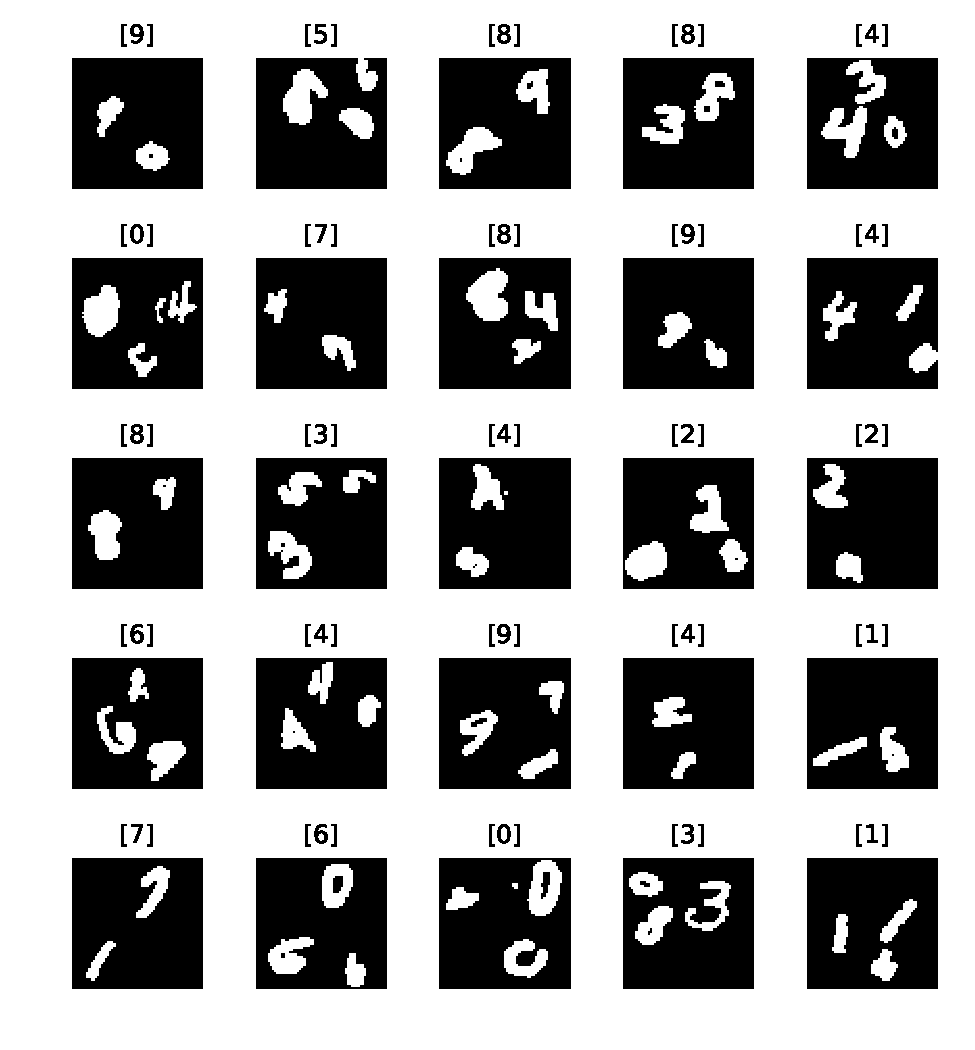
\includegraphics[width=0.5\textwidth]{figures/thresholdmedDataset.pdf}  % The printed column width is 8.4 cm.
		\caption{Output of median filter on thresholded images from Figure \ref{fig:thresholded}}
		\label{fig:thresholdmed}
	\end{center}
\end{figure}
\subsection{Biggest Number}
The output of this filter on thresholded images are shown in Figure \ref{fig:biggest}.
\begin{figure}[h]
	\begin{center}
		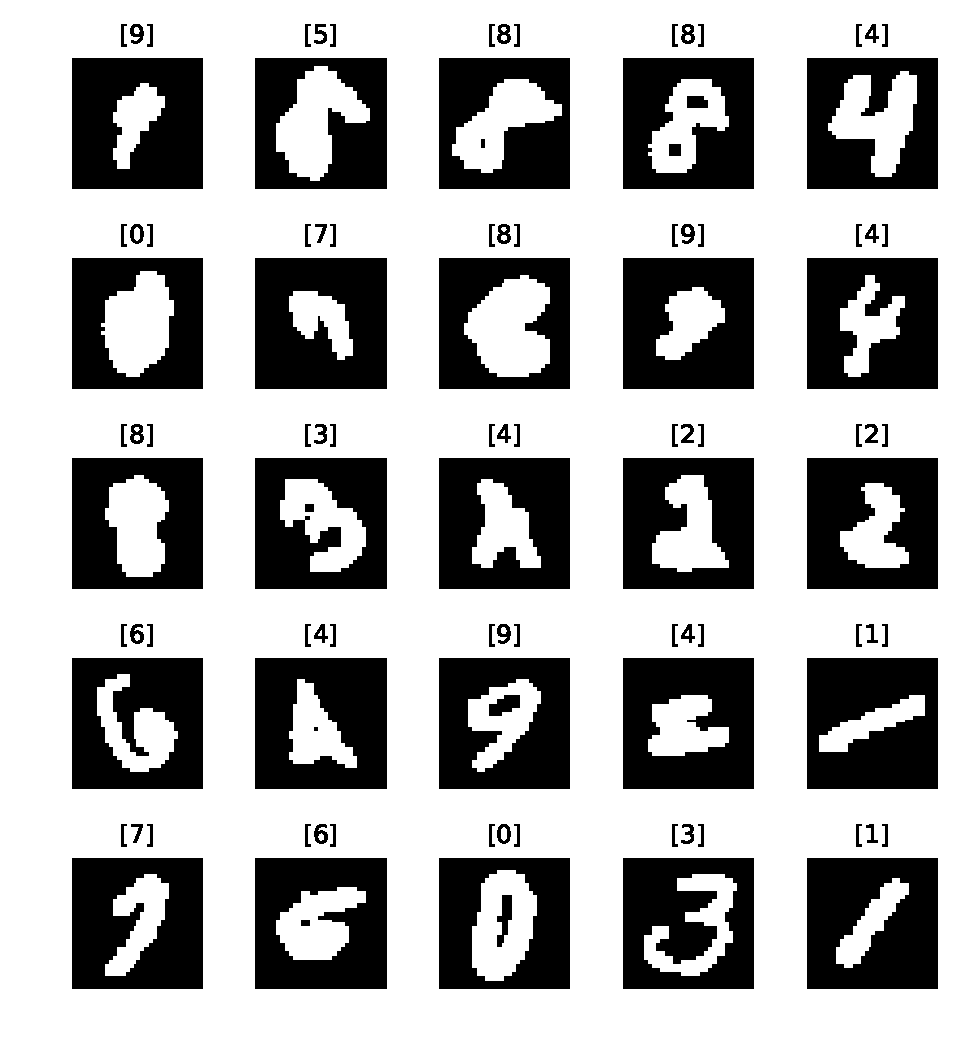
\includegraphics[width=0.5\textwidth]{figures/BiggestDataset.pdf}  % The printed column width is 8.4 cm.
		\caption{Output of biggest number filter on thresholded images from Figure \ref{fig:thresholded}}
		\label{fig:biggest}
	\end{center}
\end{figure}

\subsection{Applied Filters}
Figure \ref{fig:allFilters} shows the effect of all the above filters on one image. 
\begin{figure}[h]
	\begin{center}
		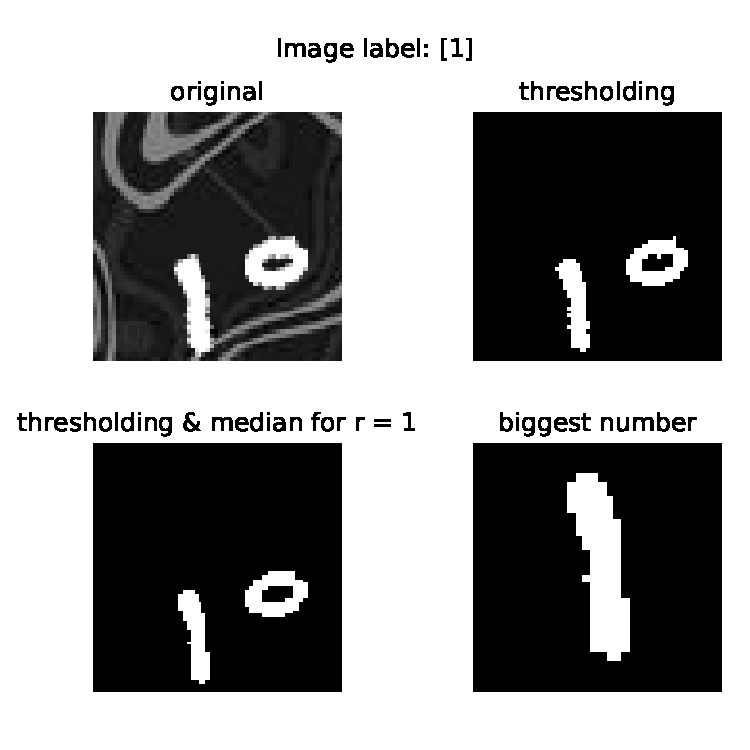
\includegraphics[width=0.5\textwidth]{figures/allDataset.pdf}  % The printed column width is 8.4 cm.
		\caption{Output of Different Filters Applied on the first image in Figure \ref{fig:original}}
		\label{fig:allFilters}
	\end{center}
\end{figure}


\section{METHODOLOGY}

To start with, we had to split the original dataset into a training and validation set. The test set was provided without labels, we had to submit our predictions to Kaggle to get the accuracy of our models. We decided to go with a simple 95/5 split for the training and validation sets. Then we applied our preprocessing steps defined in the Feature Design section to generate 2 new datasets based on the original one.

\begin{itemize}
\item For the first new dataset, we applied the threshold filter.
\item For the second dataset, we applied the threshold and median filters, then extracted the biggest number.
\end{itemize}

So we had three datasets now, each consisting of 47,500 training examples and 2,500 validation examples. We could then compare which of the preprocessing and feature selection steps work best for each model.

\subsection{Linear SVM}

\subsection{Fully Connected Neural Network}
The second algorithm we used to try to solve this classification problem is a fully connected neural network implemented from scratch using the Numpy library. A feed-forward neural network works by passing information from one layer to the next until the last layer where it makes a prediction, then it uses the error on that prediction to update its weights in order to reduce the error. The information in the network propagates forward as follow: $a_{l+1} = \sigma (W^{(l)T}a_l)$ where $a_l$ is the activation of layer $l$, $\sigma$ is a non-linear element-wise function and $W^{(l)}$ represents the weights between each neuron of layer $l$ and $l+1$. \\
We decided to keep the architecture of our neural network simple, since it is computationally expensive to train. We tried two different networks and chose the best based on the validation performance.
\begin{itemize}
\item One hidden layer with 350 neurons
\item Two hidden layers, 200 and 100 neurons respectively
\end{itemize}
Since we are dealing with a 10-class classification problem, the last layer of our network is a 10 neurons soft-max layer which outputs a probability distribution, the neuron in the final layer with the highest activation value can then be interpreted as the class with the highest probability. It then makes sense to use the cross-entropy loss function defined as
\begin{center}
$$loss = - \sum_{k=1}^{K}Y_k \log{P_k}$$
\end{center}
where $Y$ is the target and $P$ the prediction.
For both architectures, we used the $tanh$ activation function for every hidden layers and trained them on the second dataset described earlier, with the biggest number extracted, because the number of features is reduced and it's less expensive to train. We used gradient descent in conjunction with back-propagation to train the network and tried two different values for the learning rate, $0.1$ and $0.03$ and picked the one giving the best result based on the validation performance.


\subsection{Convolutional Neural Networks}
When it comes to image recognition, a convolutional neural network is one of the best options. For this project, a 10-convolutional layer CNN was built. There are 5 max pooling layers in total, one after every two convolutional layers to reduce the spatial size, each pooling layer will exactly reduce the input length and width by half. Also, there are 5 dropout regulations being applied, one after every two convolutional layers which has a drop out probability of 0.25, and one dropout after the fully connected layer which has a drop out probability of 0.5, the team believe this will prevent overfitting and reduce the interdependent learning amongst the neurons \cite{Budhiraja2016}. As shown in the Figure \ref{fig:CNNarch}, there are max pooling layers after convolutional layer 2, 4, 6, 8, 10, and dropout regulations after convolutional layer 3,5,7,9 and the fully connected layer. Activation function Rectified Linear Unit (ReLU) is used after every convolutional layer and the fully connected layer, and batch normalization is applied after the activation function.
\begin{figure*}[t]
	\begin{center}
		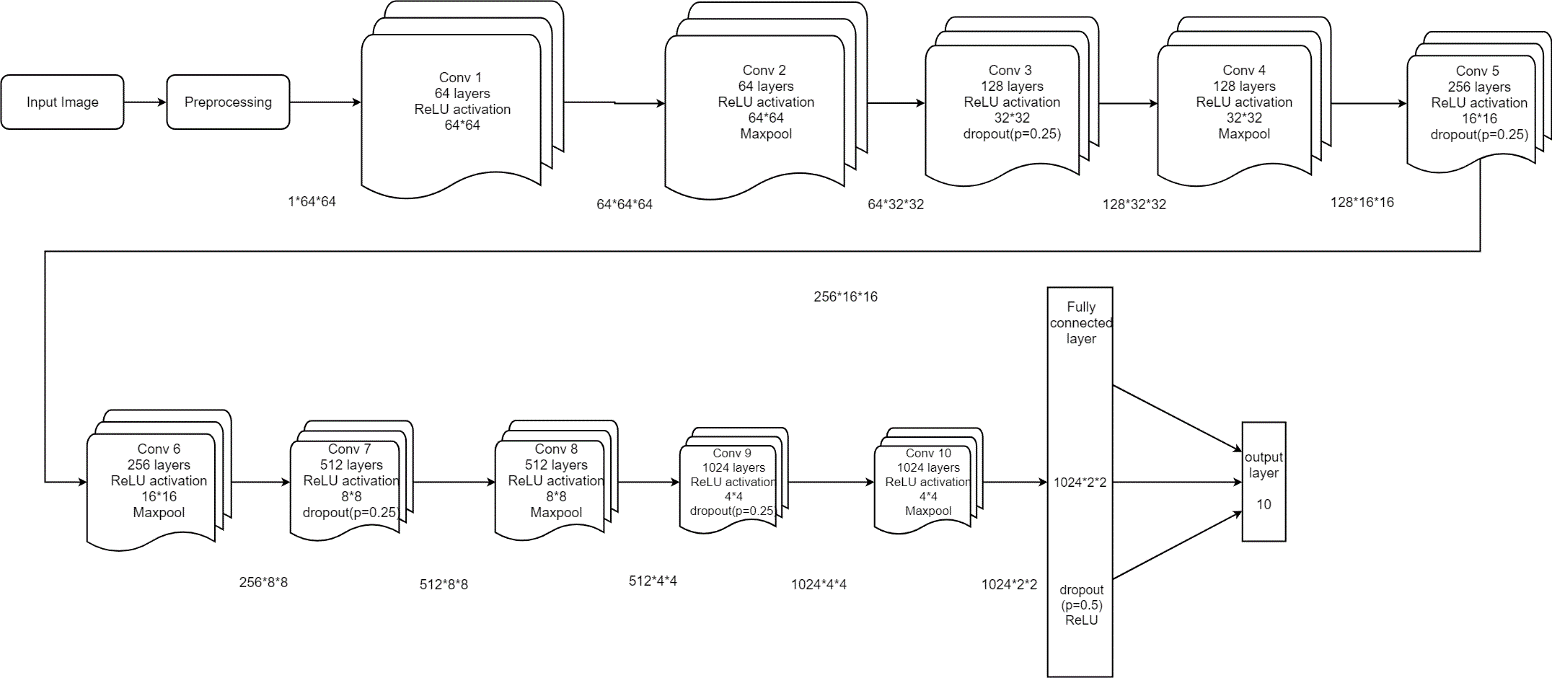
\includegraphics[width=1\textwidth]{figures/CNNflowchart.png}  % The printed column width is 8.4 cm.
		\caption{Architecture of CNN model 1}
		\label{fig:CNNarch}
	\end{center}
\end{figure*}
\begin{table*}[t]
	\centering
	\caption{hyper-parameters for CNN}
	\label{tab:hyperparams}
	\begin{tabular}{|c|c|c|c|c|c|c|l|l|l|l|l|}
		\hline
	&cov 1	&cov2	&cov 3	&cov 4	&cov 5	&cov 6	&cov 7&	cov 8&	cov 9	&cov 10&	fully connected\\\hline
number of filters&	64	&64	&128	&128	&256	&256	&512	&512&	1024	&1024	&n/a \\\hline
filter size&5&3	&3	&3	&3	&3	&3	&3	&3	&3	&n/a\\\hline
stride	&1	&1	&1	&1	&1	&1	&1	&1	&1	&1	&n/a\\\hline
zero padding &2	&1	&1	&1	&1	&1	&1	&1	&1	&1	&n/a\\\hline
max pooling	&no&	yes&	no&	yes&	no&	yes&	no&	yes&	no	&yes&n/a\\\hline
kernel size&	n/a&	2&	n/a&	2&	n/a&	2	&n/a	&2	&n/a&2&n/a\\\hline
stride	&n/a&2&	n/a	&2	&n/a&2	&n/a&2	&n/a&2&	n/a\\\hline
dropout	&no&	no&	0.25&	no	&0.25&	no&	0.25&no&0.25&no&0.5\\\hline
activation function &	ReLU&	ReLU&	ReLU&	ReLU&	ReLU&	ReLU&	ReLU&	ReLU	&ReLU&	ReLU&	ReLU\\\hline
\end{tabular}
\end{table*}
Firstly, custom training set and validation set was produced, the training set has 95\% of the data and the validation set has 5\%, the train set is set to be 95\% of the data because the CNN network have a huge amount of parameters and the team wants to use as many data as possible to train the model. Moreover, 5\% of the original training dataset is still 2500 data points, it can produce a reasonable result in a short amount of time. 
Data is fed into the CNN network a batch at a time, using the pytorch data loader class, and the batch size is set to be 300.


\section{HYPERPARAMETER SELECTION}
\subsection{Convolutional Neural Network}
As shown in the tables below there are close to 100 hyper-parameters, it is impossible to tune them all. The first filter size is chosen to be 5 as recommended by \cite{dhingra2017model}, on MNIST dataset 5x5 filter size gives the best result as shown in chart 1. And the study also showed that there is a trade of between complexity and accuracy, but if the model gets too complex without sufficient data points it has the risk of over-fitting. The number of convolution layers was chosen by gradually increasing the number of convolution layers and record the performance on the validation set. The team has find 10 convolution layers yields the best result, as shown in the chart 2, the performance increases until it reaches 12 layers, it overfits. While pooling layer was used to decreasing the number of neurons towards the bottom as suggested by \cite{lattner2016}, to be specific, after every two convolution layers a pooling layer will be employed to reduce the number of neurons by half (decrease both length and width by half and increase the depth by 2). For the number of filters of the first convolution layer (the number for the rest of the convolution will just double every two layers), different values were tested, the accuracy was improving when the number of filters go from 8 to 64 for the first convolution layer, and the improvement was not very significant after the number passed 64, and the computing time increases exponentially as the number of the filters increases. Drop out is proven to be an efficient and effective strategy to prevent overfitting \cite{srivastava2014dropout}, thus it is used as the regulation strategy for this project, 25\% of tensors get dropped every 2 convolution layers. Adam optimizer were used because it has an adaptive learning rate and momentum, it is shown to be more effective that other optimizers \cite{walia2017opt}.

\section{RESULTS}

\subsection{Linear SVM}
Using the gridsearch approach, we found that the best value of C, the error penalty of the model, is $C=1$. This model achieved an accuracy of 0.543 on the validation set. Figure \ref{fig:svmconf} shows the confusion matrix for this model.

\begin{figure}[h]
	\begin{center}
			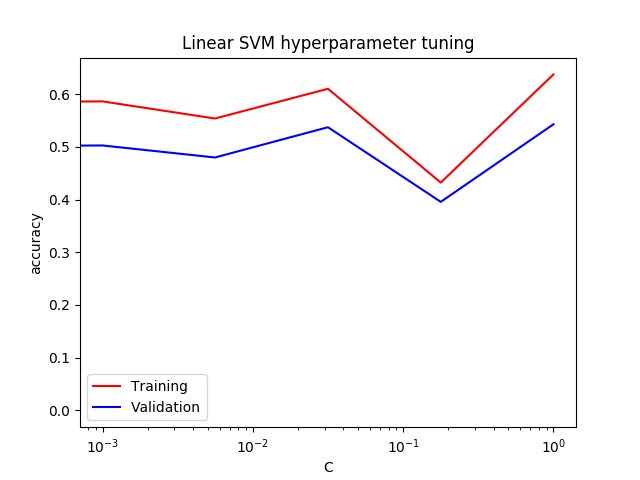
\includegraphics[width=0.5\textwidth]{figures/svm_tuning.png}  % The printed column width is 8.4 cm.
		\caption{Training and validation performance for different value of C}
		\label{fig:svmtuning}
	\end{center}
\end{figure}
\begin{figure}[h]
	\begin{center}
			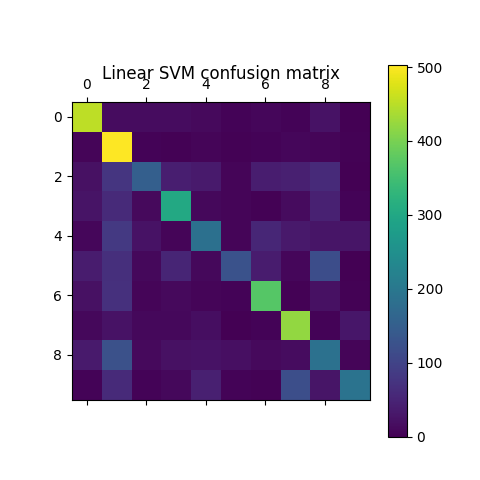
\includegraphics[width=0.5\textwidth]{figures/svm_conf.png}  % The printed column width is 8.4 cm.
		\caption{Confusion matrix for the best SVM model (targets vs outputs) with 2500 validation examples}
		\label{fig:svmconf}
	\end{center}
\end{figure}


\subsection{Fully Connected Neural Network}
Using every combinations of learning rates and layer architectures to find the best model, we found that the best accuracy on the validation data was obtained by the network composed of 1 hidden layer with 350 neurons and a learning rate of 0.03. For both network configurations that we tried, the learning rate of 0.1 was too high. The best accuracy achieved on the validation data using this network is 0.9215. Figure \ref{fig:fnnconf} show the confusion matrix of this model. We see a very high accuracy for the digits 0 and 1, which are the easiest to classify and a low accuracy for the digits 2 and 5. Also, the network tends to misclassify an 8 by a 5 quite often.

\begin{figure}[h]
	\begin{center}
			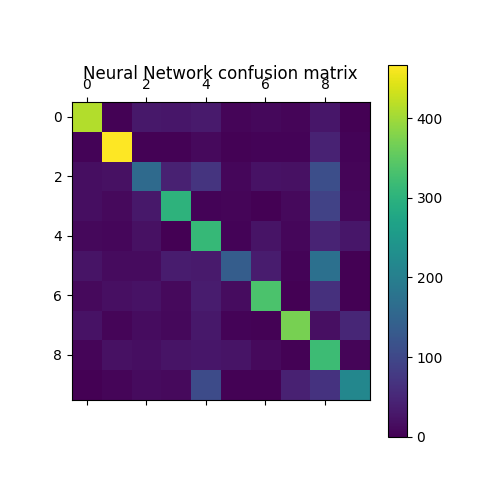
\includegraphics[width=0.5\textwidth]{figures/fnn_conf.png}  % The printed column width is 8.4 cm.
		\caption{Confusion matrix for the best FNN model (targets vs outputs)}
		\label{fig:fnnconf}
	\end{center}
\end{figure}


\subsection{Convolutional Neural Network}
Using the 10-layer CNN model have both advantages and disadvantages. The CNN network can be very accurate on image recognition tasks, our model is able to achieve an accuracy of 96.93\% training on only 47500 samples, and there is still room for improvement if more time is given. The drawback of the model is the complexity, it is slow to train and have large memory footprint, according to \cite{dhingra2017model}, there is a trade off between complexity and accuracy. Since there is no requirement about the speed or complexity in the assignment handout, a complex model with 10 layers was chosen. 

\begin{table}
	\centering
	\caption{Specification of the trained CNN models and their accuracy on Validation Set}
	\label{tab:}
	\begin{tabular}{|c|c|c|c|c|c|}
		\hline
		model	&layers&	regulation&	max pooling layer&preprocessing&accuracy\\\hline
		1&	2& n/a & 1   &	n/a		&18.9\\\hline	
		2&	3&	n/a		&1  &	n/a		&23.5\\\hline
		3&	4&	3 dropouts&2&	n/a		&60.1\\\hline
		4&	6&	3 dropouts&3&	n/a		& 84.8	\\\hline
		5&	8&	4 dropouts&4&threshold&93.4	\\\hline
		6&	10&	5 dropouts&5&threshold &96\\\hline
		7&	12&	6 dropouts&6&threshold&94.5\\\hline	
		8&	10&	7 dropouts&5&threshold&95.4\\\hline			
	\end{tabular}
\end{table}

\section{DISCUSSION}

Choosing to use the biggest number dataset for the Linear SVM training and the Fully Connected Network training was a good choice because it's the dataset with the least number of features, which can help reduce overfitting, and it makes the training faster on our computationally restricted devices. \\
For the Linear SVM model, the accuracy score is the lowest of the three approaches. This was predictable since it assumes that the data is linearly separable, which is probably not the case for this problem.\\
For the fully connected network, we see in Figure \ref{fig:fnnconf} a very high accuracy for the digits 0, 1 and 7, which are the easiest to classify because of their geometric form and a low accuracy for the digits 2 and 5. Also, the network tends to misclassify 9 by 5 and 5 by 8 quite often. In general, a lot of numbers are wrongly classified as 8 and then 5 which suggests that these are the two numbers which were not correctly learned.
The best feed forward network is the one with the most neurons, one improvement we could try is to augment the number of neurons in each layers to try to get a better validation performance on the same dataset. \\



\addtolength{\textheight}{-12cm}   % This command serves to balance the column lengths
                                  % on the last page of the document manually. It shortens
                                  % the textheight of the last page by a suitable amount.
                                  % This command does not take effect until the next page
                                  % so it should come on the page before the last. Make
                                  % sure that you do not shorten the textheight too much.

%%%%%%%%%%%%%%%%%%%%%%%%%%%%%%%%%%%%%%%%%%%%%%%%%%%%%%%%%%%%%%%%%%%%%%%%%%%%%%%%



%%%%%%%%%%%%%%%%%%%%%%%%%%%%%%%%%%%%%%%%%%%%%%%%%%%%%%%%%%%%%%%%%%%%%%%%%%%%%%%%


\section*{STATEMENT OF CONTRIBUTIONS}
Yignan implemented the convolutional neural network.
Vincent implemented the fully-connected feedforward neural
network and the linear classifiers. Hamed implemented preprocessing and tested the linear classifiers. Yignan and Vincent performed the heavy simulations using on-line clouds. All three contributed to the report with Hamed being responsible for organizing of the final report.



%%%%%%%%%%%%%%%%%%%%%%%%%%%%%%%%%%%%%%%%%%%%%%%%%%%%%%%%%%%%%%%%%%%%%%%%%%%%%%%%



\Urlmuskip=0mu plus 1mu\relax
\bibliographystyle{IEEEtran}
\bibliography{IEEEabrv,references}
%\begin{thebibliography}{99}
%
%\bibitem{c1} G. O. Young, �Synthetic structure of industrial plastics (Book style with paper title and editor),� 	in Plastics, 2nd ed. vol. 3, J. Peters, Ed.  New York: McGraw-Hill, 1964, pp. 15�64.
%\end{thebibliography}




\end{document}
